\section{Discussion}
\paragraph{Meta-PDE Methods Comparison} MAML-based Meta-PDE method outperforms LEAP-based Meta-PDE method during deployment time in both accuracy and speed. The superior performance is a results of smaller neural network architecture and fewer inner steps. The per-step and per-parameter step size serves as the main contributor to such good performance for MMAL. However, we observe that it takes longer to train the MAML-based meta-learning model because in MAML's meta-learning algorithm, we need to unroll each inner task during the training, and perform backpropagation through each inner-step through automatic differentiation. Such computation imposes a large memory constraint especially when we train the meta-learning model on a GPU with 16 GB memory. Alternatively, such computation takes a longer time when we use checkpointing to reduce the memory footprint. In two of our three experiments, we needed to use checkpoints so that we could fit the training on a single GPU. 

\begin{wrapfigure}[20]{r}{0.6\textwidth}
  \centering
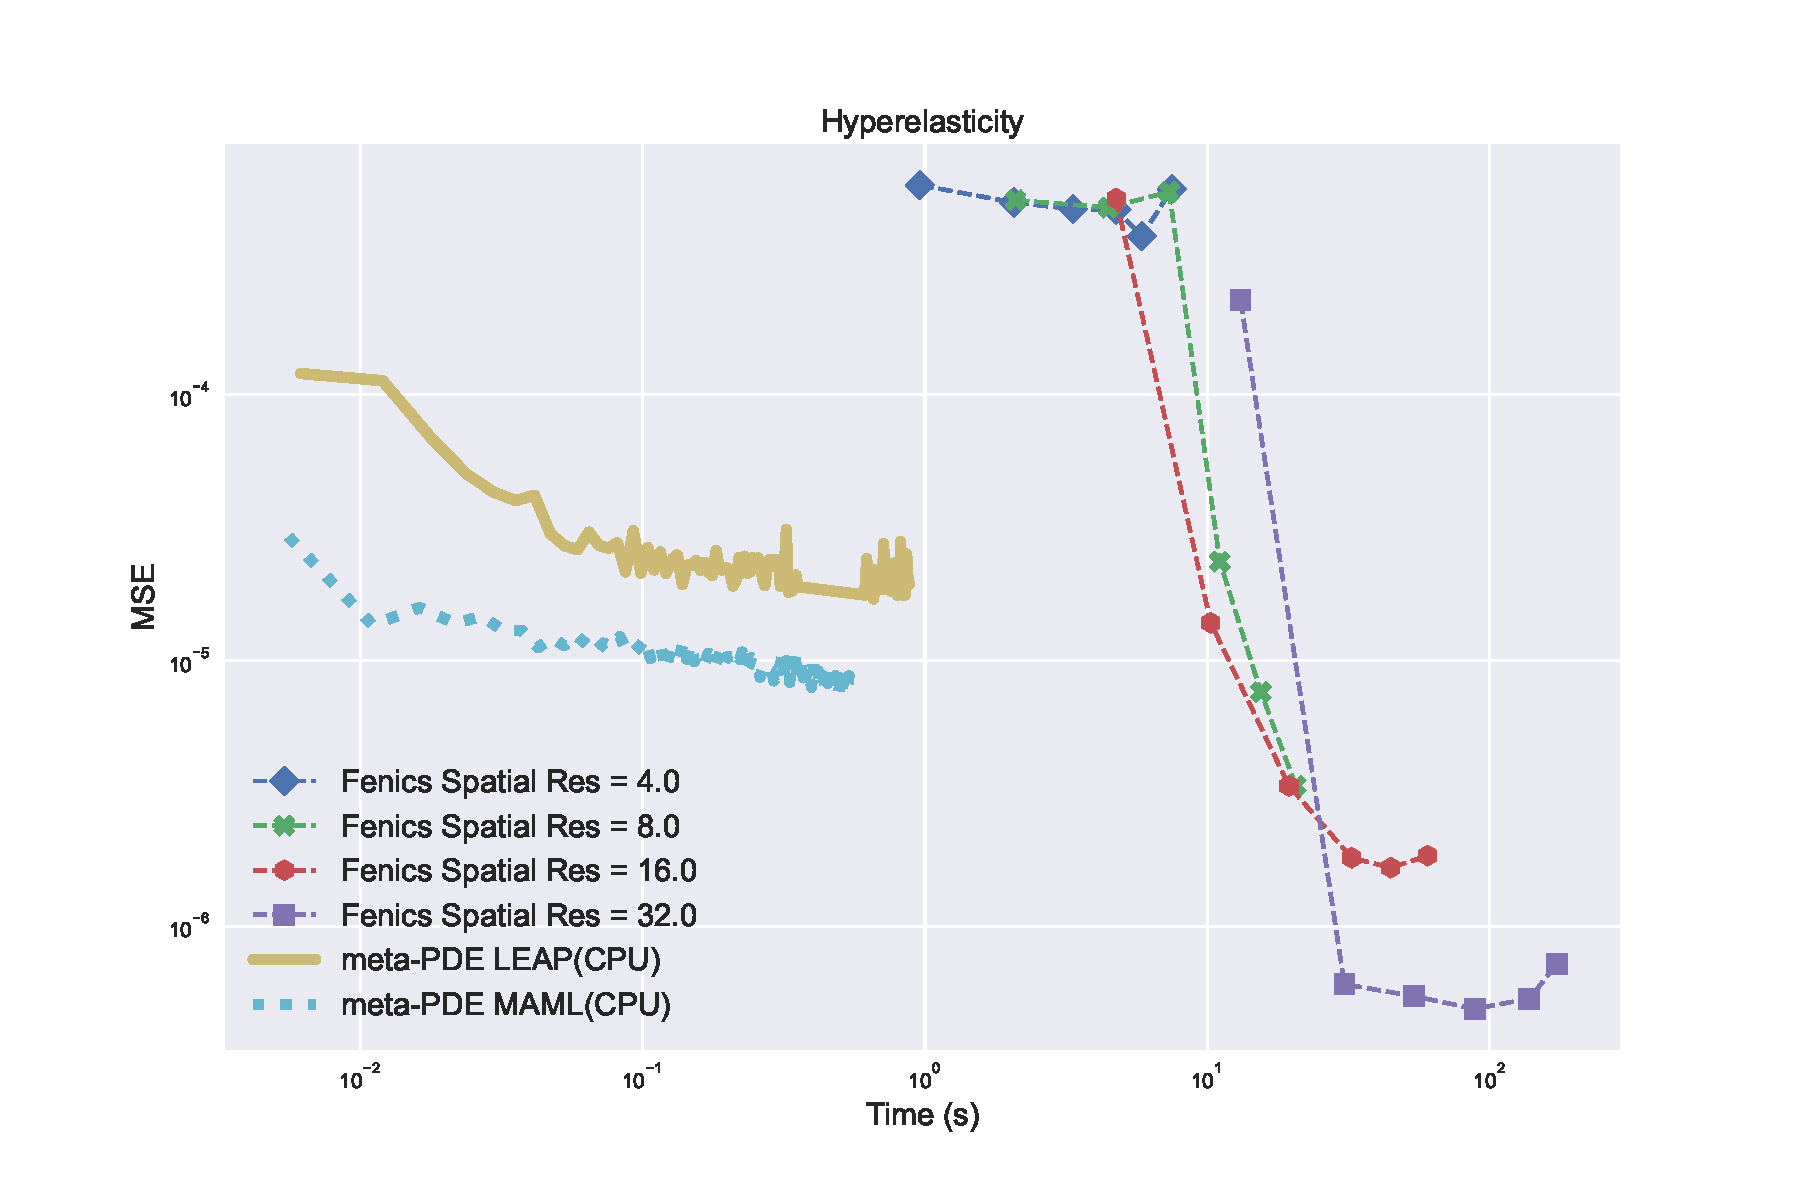
\includegraphics[width=\linewidth]{figures/hyperelasticity.pdf} 
\caption{MSE of each solution and the solving time required for the desired accuracy.}%
\label{fig:hyperelasricity_summary}%
\end{wrapfigure}

LEAP-based method, on the other hand, takes longer to adapt to new tasks due to the larger neural network sizes and more training steps. The advantage of LEAP-based Meta-PDE method lies in the meta-training process. The LEAP algorithm provides an analytical solution for the meta-gradient. The analytical solution circumvents the automatic differentiation computation needed in MAML. As a result, LEAP has a much smaller memory footprint compared to MAML. Such a computation advantage also comes at the cost of model flexibility. In particular, the MAML-based Meta-PDE method benefits from having a meta-learned per-state per-parameter step size. Having an analytical form for the meta-gradients implies that such a feature can not be easily incorporated into the LEAP algorithm. Furthermore, unlike MAML, LEAP requires the user to input the learning rate for the inner loop. Empirically, the model convergence is sensitive to the inner learning rate. As a result, the hyperparameter tuning for LEAP-based Meta-PDE method is more arduous compared to MAML. 

\paragraph{Task Domain Generalizability} In our study, we confine the meta-learner's task pool to one type of PDE, and for each type of PDE we define the task pool by having different parameterizations of the same PDE type. As we increase the task pool size, either by increasing the range of parameters or by increasing the number of paraemeters, the meta-learning tasks becomes harder. As a result, we need to use larger network architecture, increase the number of inner trainnig steps, increase meta-learner's training time to allow it to converge. The quality of the final model produced by the meta-PDE method also deteriorates. Namely, the accuracy of the solution to PDE problems after $K$ training step becomes worse. For example, in Figure \ref{fig:elasticity_flower_meta} we looked at a how different pore shapes affect the macroscopic behavior of the material. It is original problem studied by \citet{overvelde2014relating}. Neither LEAP-based Meta-PDE method nor MAML-based Meta-PDE method found a model that can solve particular instances of the PDE to a satisfactory accuracy. \\
\begin{SCfigure}[0.8][h]
  \centering
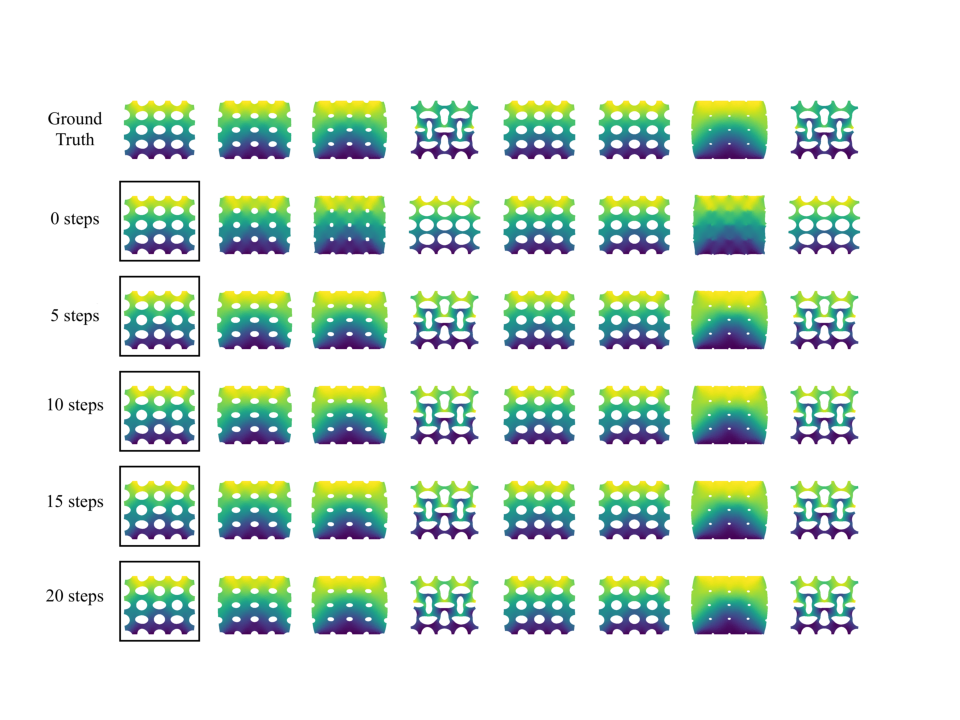
\includegraphics[width=0.6\linewidth]{figures/hyper_elasticity_circle_meta.pdf}
\caption{\small Solutions to hyper-elasticity equations with varying porous shape. Top: ground truth finite element solution. Second row: solution represented by Meta-PDE initial neural network parameters. Third row onwards: solution after each gradient step in the Meta-PDE inner loop. Looking at the bottom row, we can see that our meta-PDE based method fails to find a satisfactory solution. }%
\label{fig:elasticity_flower_meta}%
\end{SCfigure}

\paragraph{Hard-to-solve PiNNs}  
In our study, we encountered examples of PDEs such that our Meta-PDE method cannot find meaningful solutions for task pool with a meaningful size (we exclude task pools that are trivial). These PDEs include ones that PiNNs find hard to solve - Navier-Stokes Equations, 2D Burger's Equations. One possible cause for such an issue is the simplicity in our neural network architecture. In all of our experiments, We only used vanilla FCNN as our main architecture choice. However, many works have been done to tailor NN architecture design to solve these problems under the PiNN setting. For example, the attention-like model is used to fit PDE solutions in \citet{wang2020understanding}). In future study, we are interested in seeing whether one could adopt more complex NN designs into the Meta-PDE method. We are hoping to see that a better architecture design for these hard-to-solve PDEs might improve Meta-PDE's performance.